% Copyright 2026 Sreeram Anil
% SPDX-License-Identifier: CC-BY-4.0
% =============================================================================
%  Right-invariant EKF on SO(3) x R^3 — attitude (AHRS) family
% =============================================================================
\chapter{Right-Invariant Extended Kalman Filter (InvariantEKF)}
\label{ch:att-iekf}

\section*{At a glance}
\begin{tabular}{@{}l>{\raggedright\arraybackslash}p{0.76\textwidth}@{}}
Family & attitude / AHRS \\
Header & \texttt{include/estkit/attitude/iekf\_attitude.hpp} \\
Registered name & \texttt{InvariantEKF} \\
State & $\hat{\bm{q}}\in S^3$, $\hat{\bm{b}}\in\real^3$; error
 $[\bm{\xi};\bm{\beta}]\in\real^6$, $\bm{\xi}$ in the NAV frame; $\mP\in\real^{6\times6}$ \\
Cost per step & $\approx2.9\times10^3$ MACs; $\SI{1.91}{\micro\second}$/step, 608\,bytes \\
Primary references & \cite{barrau2017iekf,barrau2018review,bonnabel2007,bonnabel2009} \\
\end{tabular}

\section{Motivation and aerospace relevance}
The MEKF of Chapter~\ref{ch:att-mekf} linearises the error dynamics about the current estimate. That
is a choice, not a necessity: the error itself can be defined in more than one way, and some
definitions have dynamics that are \emph{exactly} linear no matter how large the error or how
violent the trajectory. Barrau and Bonnabel~\cite{barrau2017iekf} characterised the systems for
which this happens --- \emph{group-affine} systems on matrix Lie groups --- and showed that for them
the invariant error obeys a \emph{log-linear} differential equation whose transition matrix is
independent of the state. The consequences are two, and both are visible in the benchmark: the
filter cannot manufacture false observability from a wrong estimate, and its domain of attraction is
much larger than an ordinary EKF's.

The attitude problem is the simplest non-trivial instance. $\dot{\bm{R}}=\bm{R}[\bm{\omega}]_\times$
is equivariant under left translations $\bm{R}\mapsto\bm{R}_0\bm{R}$ --- a change of navigation frame
--- so the natural error is the \emph{right}-invariant one, and with the same input applied to truth
and estimate it is exactly conserved. That fact is one line of algebra, \eqref{eq:iekf-eta0} below,
and it replaces the MEKF's $\exp(-[\hat{\bm{\omega}}]_\times\dt)$ by the identity.

Invariant filtering is now standard in aided inertial navigation (the $SE_2(3)$ formulation of
IMU/GNSS fusion, legged-robot state estimation, visual-inertial odometry) and in spacecraft attitude
work; the attitude-only case treated here is the pedagogical core of it.

\section{Problem statement and assumptions}
The models are exactly those of Chapter~\ref{ch:att-mekf}, \eqref{eq:mekf-gyro}--\eqref{eq:mekf-meas},
and the measurement-covariance policy of \S\ref{sec:mekf-R} is reused verbatim, so that any
difference in the benchmark is attributable to the error parametrisation and to nothing else.

\begin{definition}[Invariant errors]
For $\bm{R},\hat{\bm{R}}\in SO(3)$ the \emph{right}-invariant error is
$\bm{\eta}_R=\hat{\bm{R}}\bm{R}^\T$ (invariant under $\bm{R}\mapsto\bm{R}_0\bm{R}$,
$\hat{\bm{R}}\mapsto\bm{R}_0\hat{\bm{R}}$ up to conjugation, and a NAV-frame object) and the
\emph{left}-invariant error is $\bm{\eta}_L=\bm{R}^\T\hat{\bm{R}}$ (a BODY-frame object). The MEKF's
$\delta\bm{\theta}$ is the logarithm of $\bm{\eta}_L^{-1}$.
\end{definition}

\section{Derivation}

\subsection{Why the right-invariant error is the right one here}
Assume for a moment a perfect gyro, $\hat{\bm{\omega}}=\bm{\omega}$. Then
$\dot{\bm{R}}=\bm{R}[\bm{\omega}]_\times$ and $\dot{\hat{\bm{R}}}=\hat{\bm{R}}[\bm{\omega}]_\times$,
so, using $\dot{(\bm{R}^\T)}=-[\bm{\omega}]_\times\bm{R}^\T$,
\begin{equation}
\dot{\bm{\eta}}_R = \dot{\hat{\bm{R}}}\bm{R}^\T + \hat{\bm{R}}\dot{(\bm{R}^\T)}
 = \hat{\bm{R}}[\bm{\omega}]_\times\bm{R}^\T - \hat{\bm{R}}[\bm{\omega}]_\times\bm{R}^\T = \bm{0}.
\label{eq:iekf-eta0}
\end{equation}
The right-invariant error is \emph{exactly constant}: no linearisation, no dependence on
$\bm{\omega}$, no dependence on how large the error is. This is the log-linear property of
Barrau and Bonnabel~\cite[Thm.~1]{barrau2017iekf} in its simplest form; the attitude block of the
error-propagation matrix is the identity. Contrast the MEKF, whose body-frame error obeys
$\dot{\delta\bm{\theta}}=-[\hat{\bm{\omega}}]_\times\delta\bm{\theta}+\dots$ --- correct only to
first order, and driven by the estimated (hence possibly wrong) rate.

Note that the \emph{left}-invariant error would \emph{not} be conserved here, because the dynamics
are right-multiplicative; the choice of error must match the symmetry of the dynamics, and the
symmetry is fixed by the fact that $\bm{\omega}$ is a body rate.

\subsection{The imperfect IEKF: adding the gyro bias}
A bias breaks the picture, because $\bm{b}$ does not live in $SO(3)$ and the augmented system is no
longer group-affine; this is the ``imperfect IEKF'' of \cite[Sec.~V]{barrau2017iekf}. Repeating
\eqref{eq:iekf-eta0} with $\hat{\bm{\omega}}=\bm{\omega}_y-\hat{\bm{b}}$,
$\bm{\omega}=\bm{\omega}_y-\bm{b}-\bm{n}_v$ and $\bm{\beta}=\bm{b}-\hat{\bm{b}}$,
\begin{equation}
\dot{\bm{\eta}}_R = \hat{\bm{R}}\big[\hat{\bm{\omega}}-\bm{\omega}\big]_\times\bm{R}^\T
 = \hat{\bm{R}}\big[\bm{\beta}+\bm{n}_v\big]_\times\hat{\bm{R}}^\T\,\bm{\eta}_R
 = \big[\hat{\bm{R}}(\bm{\beta}+\bm{n}_v)\big]_\times\,\bm{\eta}_R ,
\label{eq:iekf-etadot}
\end{equation}
using $\bm{A}[\bm{v}]_\times\bm{A}^\T=[\bm{A}\bm{v}]_\times$ for $\bm{A}\in SO(3)$. Writing
$\bm{\eta}_R=\exp([\bm{\xi}]_\times)$ with $\bm{\xi}\in\real^3$ a \emph{navigation-frame} rotation
vector, \eqref{eq:iekf-etadot} gives to first order in $\bm{\xi}$
\begin{equation}
\dot{\bm{\xi}} = \hat{\bm{R}}\big(\bm{\beta}+\bm{n}_v\big),
\qquad
\dot{\bm{\beta}} = \bm{n}_u ,
\label{eq:iekf-err}
\end{equation}
so
\begin{equation}
\mF = \begin{bmatrix}\bm{0} & \hat{\bm{R}}\\ \bm{0}&\bm{0}\end{bmatrix},
\qquad
\bm{\Phi}=\exp(\mF\dt)=\begin{bmatrix}\bm{I} & \hat{\bm{R}}\dt\\ \bm{0}&\bm{I}\end{bmatrix}
\quad\text{exactly, since } \mF^2=\bm{0}.
\label{eq:iekf-Phi}
\end{equation}
Three things are worth saying about \eqref{eq:iekf-Phi}. \emph{(i)} The attitude block is
\emph{exactly} the identity --- there is no $\exp(-[\hat{\bm{\omega}}]_\times\dt)$ and therefore no
trajectory dependence whatsoever in the attitude error propagation. \emph{(ii)} The only state
dependence left is the rotation $\hat{\bm{R}}$ in the coupling block, which merely expresses that
the bias is a body-frame quantity while $\bm{\xi}$ is a navigation-frame one. \emph{(iii)} The
matrix exponential is exact, not truncated, because $\mF$ is nilpotent.

The discrete process noise follows from van Loan~\cite{vanloan1978} as in \eqref{eq:mekf-Q};
$\hat{\bm{R}}\hat{\bm{R}}^\T=\bm{I}$ removes the rotation from the diagonal blocks and leaves it in
the cross term:
\begin{equation}
\mQ_d=\begin{bmatrix}
 \big(\sigma_v^2\dt+\tfrac13\sigma_u^2\dt^3\big)\bm{I} & \tfrac12\sigma_u^2\dt^2\,\hat{\bm{R}}\\[2pt]
 \tfrac12\sigma_u^2\dt^2\,\hat{\bm{R}}^\T & \sigma_u^2\dt\,\bm{I}\end{bmatrix} .
\label{eq:iekf-Q}
\end{equation}
The sign of the cross block is opposite to the MEKF's \eqref{eq:mekf-Q}, because $\mF_{12}$ is
$+\hat{\bm{R}}$ here and $-\bm{I}$ there.

\subsection{Right-invariant observations and the invariant innovation}
Gravity and the magnetic field are observed as $\bm{y}=\bm{R}^\T\bm{r}+\bm{n}$ with $\bm{r}$ a
\emph{known navigation} vector. In the language of \cite{barrau2017iekf} these are
\emph{right-invariant} observations: they are of the form $\bm{y}=\chi^{-1}\bm{r}$ and are therefore
compatible with the right-invariant error. The invariant innovation is formed by carrying the
measurement into the navigation frame,
\begin{equation}
\bm{z} = \hat{\bm{R}}\bm{y} - \bm{r}
 = \bm{\eta}_R\bm{r} - \bm{r} + \hat{\bm{R}}\bm{n}
 = \bm{\xi}\times\bm{r} + \hat{\bm{R}}\bm{n} + O(\norm{\bm{\xi}}^2)
 = -[\bm{r}]_\times\bm{\xi} + \hat{\bm{R}}\bm{n} + O(\norm{\bm{\xi}}^2),
\label{eq:iekf-z}
\end{equation}
hence
\begin{equation}
\mH = \big[\,-[\bm{r}]_\times\quad \bm{0}_{3\times3}\,\big],
\qquad
\operatorname{cov}\!\big(\hat{\bm{R}}\bm{n}\big)=\hat{\bm{R}}\,\sigma^2\bm{I}\,\hat{\bm{R}}^\T=\sigma^2\bm{I} .
\label{eq:iekf-H}
\end{equation}
\begin{remark}[The state has disappeared from the filter gain]
$\mH$ in \eqref{eq:iekf-H} depends only on the \emph{known} reference $\bm{r}$ --- not on
$\hat{\bm{q}}$, not on the trajectory --- and for isotropic sensor noise neither does the
measurement covariance. Combined with $\bm{\Phi}_{11}=\bm{I}$, this means the entire covariance
recursion of the attitude block is deterministic: $\mP$, $\mS$ and $\mK$ evolve along a
trajectory-independent path. An ordinary EKF's $\mH=[\hat{\bm{R}}^\T\bm{r}]_\times$ is evaluated at
the estimate, so a wrong estimate produces a wrong gain and, worse, a covariance that reflects the
observability of a system the vehicle is not on --- the ``false observability'' that makes EKFs
inconsistent after a large heading error. The invariant filter cannot do this.
\end{remark}

\subsection{Update and reset}
The Kalman update is the usual one on $[\bm{\xi};\bm{\beta}]$ with the stacked accelerometer and
magnetometer blocks, in Joseph form. Since $\bm{\eta}_R=\hat{\bm{R}}\bm{R}^\T=\exp([\bm{\xi}]_\times)$
implies $\bm{R}=\exp(-[\bm{\xi}]_\times)\hat{\bm{R}}$, the correction is a \emph{left}
(navigation-frame) multiplication,
\begin{equation}
\hat{\bm{q}}\leftarrow \exp\!\big(-\bm{\xi}^+\big)\otimes\hat{\bm{q}},
\qquad
\hat{\bm{b}}\leftarrow \hat{\bm{b}}+\bm{\beta}^+ ,
\label{eq:iekf-reset}
\end{equation}
where the MEKF's reset \eqref{eq:mekf-reset} is a right multiplication. That single difference ---
which side the correction is applied on, and correspondingly in which frame the error is
expressed --- is the whole of the invariant EKF.

A second-order reset transform for the cross-covariance (the bias error is body-referenced and
$\hat{\bm{R}}$ has just changed) is $O(\norm{\bm{\xi}^+}^2)$ and is omitted, as in
\cite{barrau2018review}.

\section{Algorithm}
\begin{algorithm}[H]
\caption{Right-invariant EKF --- one sampling period}
\begin{algorithmic}[1]
\Require $\hat{\bm{q}},\hat{\bm{b}},\mP$; $\bm{\omega}_y,\bm{f},\bm{m}$
\State $\hat{\bm{\omega}}\gets\bm{\omega}_y-\hat{\bm{b}}$;\;
       $\hat{\bm{q}}\gets\hat{\bm{q}}\otimes\exp(\hat{\bm{\omega}}\dt)$, normalise;\;
       $\hat{\bm{R}}\gets\bm{R}(\hat{\bm{q}})$
\State $\bm{\Phi}\gets\big[\begin{smallmatrix}\bm{I}&\hat{\bm{R}}\dt\\ \bm{0}&\bm{I}\end{smallmatrix}\big]$;\;
       $\mQ_d\gets$ \eqref{eq:iekf-Q};\; $\mP\gets\bm{\Phi}\mP\bm{\Phi}^\T+\mQ_d$; symmetrise
\State $\bm{z}\gets\big[\hat{\bm{R}}\bm{f}-\bm{r}_a;\ \hat{\bm{R}}\bm{m}-\bm{r}_m\big]$
       \Comment{invariant innovation, NAV frame}
\State $\mH\gets\big[\begin{smallmatrix}-[\bm{r}_a]_\times&\bm{0}\\ -[\bm{r}_m]_\times&\bm{0}\end{smallmatrix}\big]$
       \Comment{constant matrices}
\State $\bm{\Sigma}\gets$ \eqref{eq:mekf-R}--\eqref{eq:mekf-sx} with editing
\State $\mK\gets\mP\mH^\T(\mH\mP\mH^\T+\bm{\Sigma})\inv$;\;
       $[\bm{\xi}^+;\bm{\beta}^+]\gets\mK\bm{z}$
\State $\mP\gets(\mI-\mK\mH)\mP(\mI-\mK\mH)^\T+\mK\bm{\Sigma}\mK^\T$; symmetrise
\State $\hat{\bm{q}}\gets\exp(-\bm{\xi}^+)\otimes\hat{\bm{q}}$, normalise;\;
       $\hat{\bm{b}}\gets\operatorname{clamp}(\hat{\bm{b}}+\bm{\beta}^+)$
\Ensure $\hat{\bm{q}},\hat{\bm{b}},\mP$
\end{algorithmic}
\end{algorithm}

\section{Application to the benchmark flight}
Identical to the MEKF, deliberately: $\mP_0=\diag((30^\circ)^2\bm{I},(\SI{3}{\degree\per\second})^2\bm{I})$,
$\sigma_v,\sigma_u$ from the configuration through \eqref{eq:mekf-units},
$\sigma_{a,\text{extra}}=\SI{0.5}{\metre\per\second\squared}$,
$\sigma_{m,\text{extra}}=\SI{1.5}{\micro\tesla}$, $V_{\text{ref}}=\SI{45}{\metre\per\second}$,
$\varpi=\SI{0.02}{\radian\per\second}$, editing at $\SI{1}{\metre\per\second\squared}$ and
$\SI{3}{\micro\tesla}$, Joseph form. Nothing was re-tuned for this filter, so the comparison in the
results is a clean A/B on the error parametrisation.

\section{Implementation notes}
The cost is the same $\approx2.9\times10^3$ multiply--adds as the MEKF, and in fact measurably
lower in practice ($\SI{1.91}{\micro\second}$/step against $\SI{2.04}{}$, a $6\,\%$ saving) because
$\bm{\Phi}$ is assembled from a rotation matrix that is needed anyway and requires no
$\sin/\cos$ evaluation --- the closed-form $\bm{\Phi}_{11},\bm{\Phi}_{12}$ of the MEKF,
\eqref{eq:mekf-phi11}--\eqref{eq:mekf-phi12}, are gone. \code{sizeof} is 608\,bytes, identical.

A production implementation can exploit more: $\mH$ in \eqref{eq:iekf-H} is a pair of \emph{constant}
skew matrices, so $\mH\mP\mH^\T$ and $\mP\mH^\T$ are cross products rather than general matrix
products, and if $\bm{\Sigma}$ were constant the whole gain sequence could be precomputed offline
(it is not here, because of the adaptive $\bm{\Sigma}$ of \S\ref{sec:mekf-R}).

Numerical hygiene: as for the MEKF --- symmetrisation after both updates, Joseph form, finiteness
checks on $\mK$ and on the correction, quaternion renormalisation after the reset, bias clamped to
$\pm\SI{15}{\degree\per\second}$. \code{Quat::exp} falls back to its first-order form below
$10^{-9}$\,rad. The single-precision build reproduces the double-precision mission RMS to four digits.

\section{Benchmark results}
% Copyright 2026 Sreeram Anil
% SPDX-License-Identifier: CC-BY-4.0
\begin{table}[H]\centering\footnotesize\setlength{\tabcolsep}{3.5pt}\caption{InvariantEKF: attitude benchmark (mean over seeds; all angles in degrees; $t_\mathrm{conv}$: first time the attitude error stays below 2$^\circ$ for 30\,s; bias RMSE in deg/s; 608 bytes of state).}\label{tab:imu_InvariantEKF}
\begin{tabular}{lrrrrrrrrcr}\toprule scenario & RMS & roll & pitch & yaw & max & RMS$_\mathrm{ss}$ & $t_\mathrm{conv}$ [s] & bias RMSE & lost & ns/step \\ \midrule
nominal & 2.49 & 0.84 & 0.68 & 2.24 & 15.1 & 3.08 & 0 & 0.17 & no & 1910 \\
init\_error & 2.49 & 0.84 & 0.68 & 2.24 & 15.1 & 3.08 & 0 & 0.18 & no & 1910 \\
gyro\_bias & 2.49 & 0.84 & 0.68 & 2.24 & 15.1 & 3.08 & 2 & 0.19 & no & 1934 \\
mag\_disturbance & 2.88 & 0.85 & 0.68 & 2.66 & 15.9 & 3.08 & 0 & 0.19 & no & 1901 \\
vibration & 2.14 & 0.71 & 0.57 & 1.93 & 16.6 & 2.52 & 11 & 0.15 & no & 1906 \\
high\_dynamics & 3.30 & 1.15 & 0.76 & 3.02 & 12.7 & 3.90 & 222 & 0.20 & no & 1909 \\
\bottomrule\end{tabular}\end{table}

\begin{figure}[H]\centering
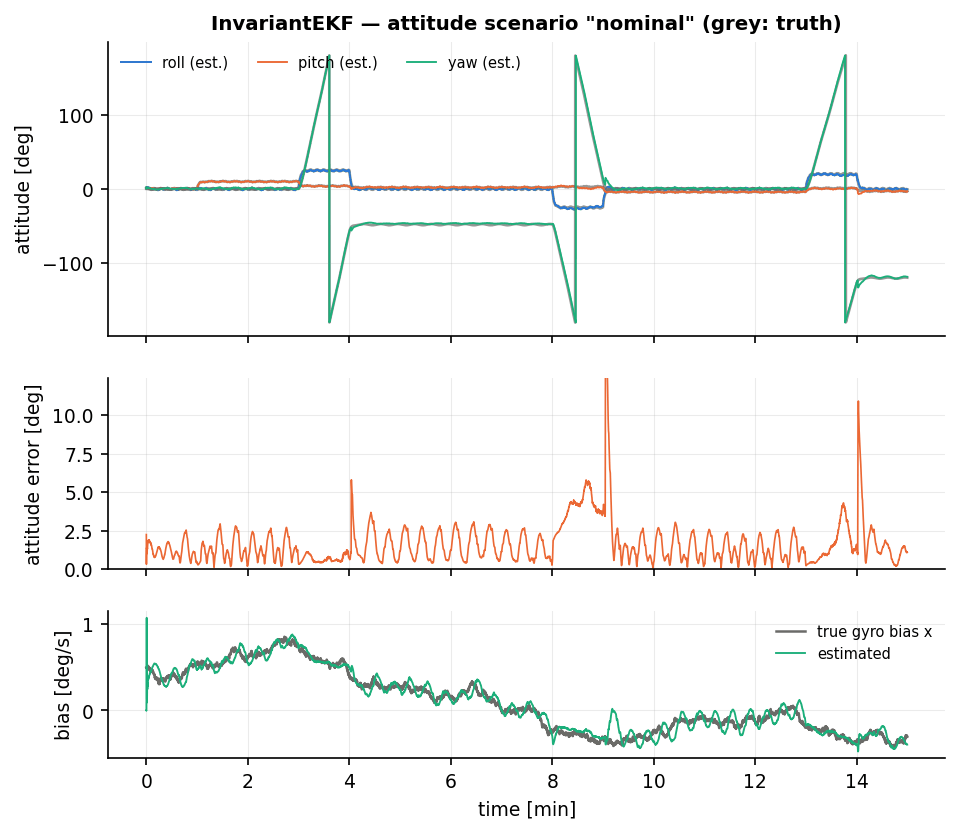
\includegraphics[width=\textwidth]{figures/imu_InvariantEKF_nominal.png}
\caption{Invariant EKF on the nominal mission.}
\end{figure}
\begin{figure}[H]\centering
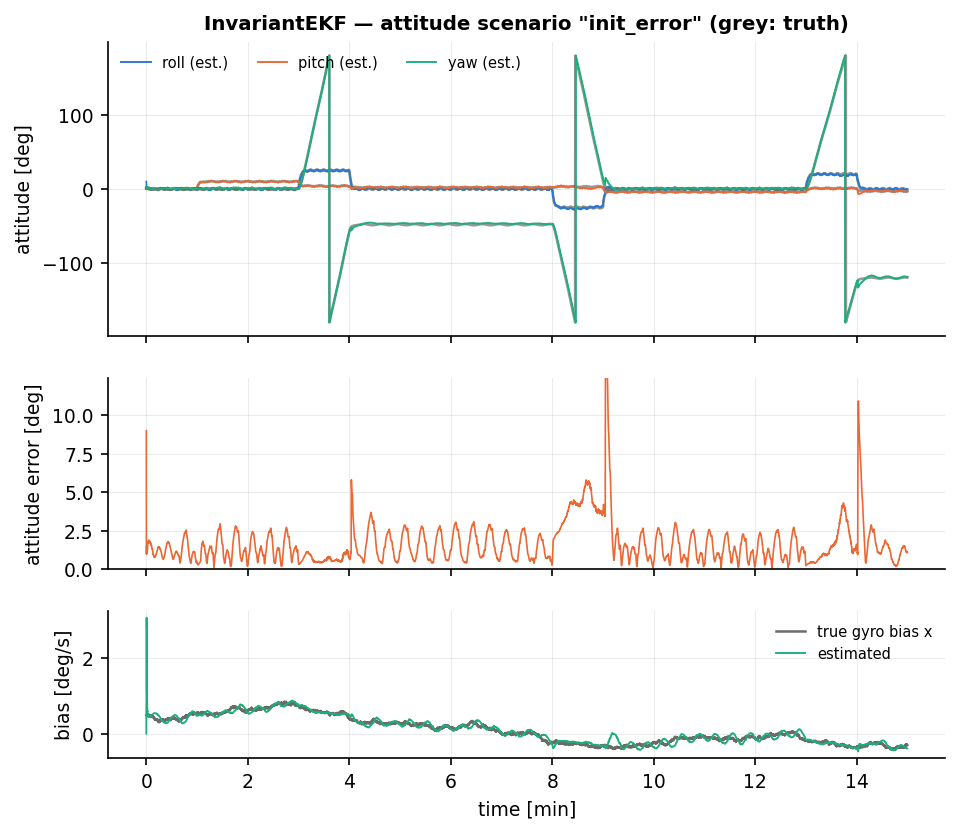
\includegraphics[width=\textwidth]{figures/imu_InvariantEKF_init_error.png}
\caption{Invariant EKF with a $46.6^\circ$ initial attitude error: the transient lasts one sample.}
\end{figure}

In steady state the two six-state filters are indistinguishable, as they should be --- at
$\norm{\bm{\xi}}<1^\circ$ the two linearisations agree to second order. Mission RMS across the six
scenarios in table order is $2.49/2.49/2.49/2.88/2.14/\SI{3.30}{\degree}$, against the MEKF's
$2.48/2.50/2.48/2.86/2.14/\SI{3.33}{\degree}$; on nominal roll $0.84$, pitch $0.68$, yaw
$\SI{2.24}{\degree}$, $\text{RMS}_{\text{ss}}=\SI{3.08}{\degree}$, peak $\SI{15.1}{\degree}$, bias
RMSE $\SI{0.17}{\degree\per\second}$, never lost, and the cost is
$\SI{1.91}{\micro\second}$/step. Per phase on nominal (seed~1),
\[
1.30\;/\;1.50\;/\;1.16\;/\;1.74\;/\;4.63\;/\;1.91\;/\;2.78\;/\;1.86\ \SI{}{\degree},
\]
i.e. within $\SI{0.1}{\degree}$ of the MEKF in every phase. The invariant formulation is \emph{not} a free accuracy improvement in the regime the
mission spends its time in, and saying otherwise would be dishonest.

Two differences do survive into the three-seed table, both small and both in the predicted
direction. On \texttt{init\_error} the invariant filter reports $t_{\text{conv}}=\SI{0}{\second}$
and a bias RMSE of $\SI{0.18}{\degree\per\second}$ --- identical to its own nominal row --- while the
MEKF slips to $\SI{3}{\second}$ and $\SI{0.25}{\degree\per\second}$: the MEKF's initial transient
leaks into its bias estimate and the invariant filter's does not. On \texttt{high\_dynamics}, where
the angular rates are tripled and the MEKF's $\exp(-[\hat{\bm{\omega}}]_\times\dt)$ has the most work
to do, the invariant filter is marginally better ($3.30$ against $\SI{3.33}{\degree}$).

\paragraph{Where it does pay: large initial error.} The benchmark's \texttt{init\_error} scenario is
too gentle to separate the two in mission RMS (the transient lasts under a second out of
$\SI{900}{\second}$). Measured directly, starting the two filters from a deliberately wrong attitude
on the nominal data (seed~1) and recording the time to bring the total angular error below a
threshold:
\begin{center}
\begin{tabular}{@{}lrrrrr@{}}
\toprule
initial error & \multicolumn{2}{c}{$t(<5^\circ)$ [s]} & \multicolumn{2}{c}{$t(<2^\circ)$ [s]} & RMS over first $\SI{30}{\second}$ \\
\cmidrule(lr){2-3}\cmidrule(lr){4-5}\cmidrule(lr){6-6}
 & MEKF & IEKF & MEKF & IEKF & MEKF\,/\,IEKF [deg] \\
\midrule
$0^\circ$      & $0.00$ & $0.00$ & $0.01$ & $0.01$ & $1.32$\,/\,$1.32$ \\
$46.6^\circ$   & $0.17$ & $\bm{0.01}$ & $0.61$ & $\bm{0.04}$ & $2.71$\,/\,$\bm{1.33}$ \\
$78.5^\circ$   & $2.67$ & $\bm{0.04}$ & $3.69$ & $\bm{1.15}$ & $3.52$\,/\,$\bm{1.57}$ \\
$90.0^\circ$   & $0.08$ & $0.07$ & $1.57$ & $\bm{0.16}$ & $1.59$\,/\,$1.54$ \\
\bottomrule
\end{tabular}
\end{center}
From $46.6^\circ$ the invariant filter is inside $5^\circ$ after \emph{one sample}
($\SI{0.01}{\second}$) where the MEKF needs 17; from $78.5^\circ$ the ratio is 67. The reason is
exactly \eqref{eq:iekf-eta0} and \eqref{eq:iekf-H}: the propagation of the attitude error involves
no approximation at all, and the measurement Jacobian is evaluated at the known reference rather
than at the (badly wrong) estimate, so the first gain is the \emph{correct} gain rather than one
computed for an attitude the vehicle is nowhere near. The first-$\SI{30}{\second}$ RMS, a fairer
statistic than a threshold crossing, is $\SI{1.57}{\degree}$ against $\SI{3.52}{\degree}$ at
$78.5^\circ$ --- and the invariant filter's $\SI{1.33}{\degree}$ at $46.6^\circ$ is the same as its
own value from a \emph{perfect} start, which is as strong a statement of the log-linear property as
this benchmark can make.

\paragraph{Where it does not pay.} With a deliberately over-loose bias prior,
$\mP_{0,bb}=(\SI{10}{\degree\per\second})^2\bm{I}$, the invariant filter is \emph{worse} than the
MEKF on two scenarios ($9.21$ versus $\SI{8.77}{\degree}$ on \texttt{init\_error}, and $9.95$ versus
$\SI{1.84}{\degree}$ on \texttt{vibration}); at the registered $\SI{3}{\degree\per\second}$ the two
agree to $\SI{0.03}{\degree}$. The mechanism is the one the theory warns about: the bias is
\emph{not} part of the group, so \eqref{eq:iekf-Phi} is only ``imperfectly'' invariant, and the
cross-block $\hat{\bm{R}}\dt$ maps a body-referenced bias error into a navigation-referenced
attitude error through a rotation that itself turns by $312^\circ$ during the mission. A large
initial bias uncertainty is therefore smeared over navigation directions in a way the MEKF's
constant $-\bm{I}\dt$ coupling avoids. The invariance argument buys exactness in the attitude block
and nothing in the bias block, and it is honest to say so.

\paragraph{Everything else is shared.} Because the two filters use the same $\bm{\Sigma}$ policy,
the ablations of Chapter~\ref{ch:att-mekf} carry over unchanged: with editing disabled the invariant
filter gives $\SI{7.81}{\degree}$ against the MEKF's $\SI{7.80}{\degree}$; with no manoeuvre bound
both are near $\SI{19.3}{\degree}$. \texttt{vibration} is again the best scenario
($\SI{2.14}{\degree}$) and \texttt{high\_dynamics} the worst ($\SI{3.30}{\degree}$). The
$\SI{0.65}{\degree}$ hard-iron heading floor and the $\tan I=2.14$ dip amplification quantified in
Chapter~\ref{ch:att-mekf} apply identically here.

\section{Summary}
The right-invariant EKF is the MEKF with the attitude error moved from the body frame to the
navigation frame. One line of algebra, \eqref{eq:iekf-eta0}, then makes the attitude-error
propagation exact and the measurement Jacobian \eqref{eq:iekf-H} state-independent, at identical
cost --- slightly cheaper here, since the closed-form transition matrix is replaced by a rotation
that was needed anyway. Use it whenever the initial attitude may be badly wrong (coarse alignment,
post-fault recovery, in-flight re-initialisation), whenever consistency of the reported covariance
matters, or whenever the vehicle is highly dynamic: from a $78.5^\circ$ initial error it converges
$67$ times faster than the MEKF and more than halves the first-$\SI{30}{\second}$ RMS. Do not expect it to
improve steady-state accuracy --- here it is within $\SI{0.03}{\degree}$ of the MEKF on every
scenario, and both are beaten on \texttt{nominal} by a $\SI{132}{\nano\second}$ gated Mahony filter
(Chapter~\ref{ch:att-mahony}) --- and do not expect the invariance to extend to the bias, which is
not a group element: with a very loose bias prior the invariant filter is the more fragile of the
two.
